\subsection{Replicate}
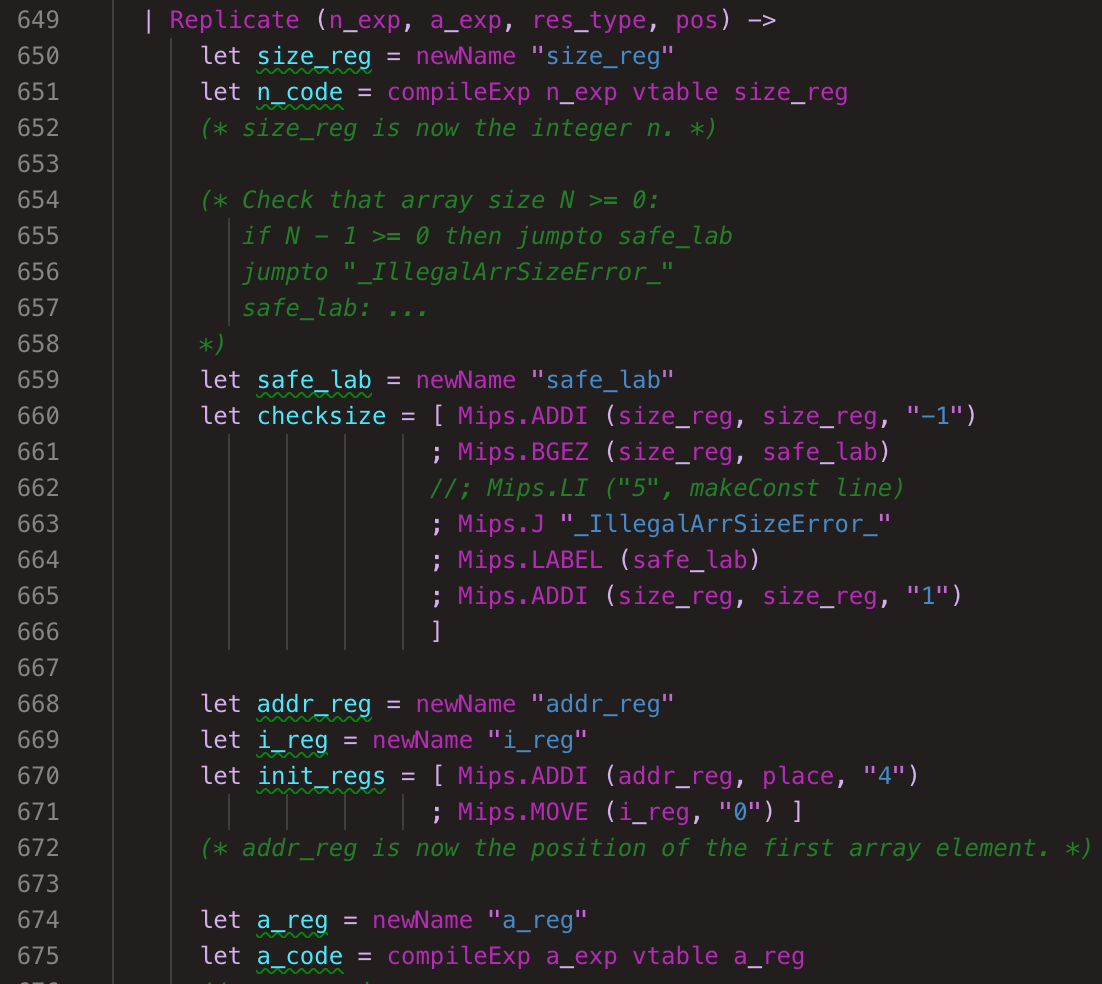
\includegraphics[width=\linewidth]{Materials/CodeGen/ReplicateIntro}
To implement replicate we first check if the given '\textit{n expression}' is greater than zero, and then we create a new array of size \textit{n} (lines 652-669). Then we create a register \textit{addr\_reg} which points to the first entry in the new array and we create another register \textit{a\_reg} which contains our given input which we want to replicate.\\
The idea is we create a loop and in each iteration we put the value of \textit{a\_reg} into the new array.\\
First we save the value of \textit{a\_reg} in \textit{addr\_reg} such that the entry in the new array which \textit{addr\_reg} points to now contains the replicated value. Then we add to \textit{addr\_reg} so it points to the next entry and we update the loop counter \textit{i\_reg} and start the loop anew. All of this is done on lines 682-701.\\
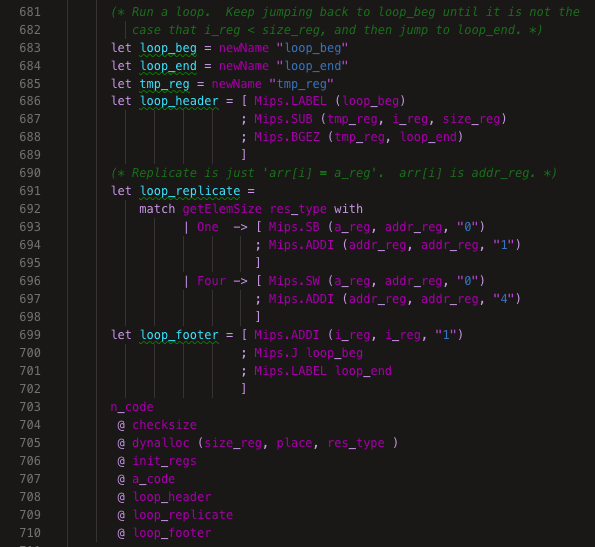
\includegraphics[width=\linewidth]{Materials/CodeGen/Replicate1}
